\documentclass{article}
%\documentclass[11pt]{article}
%\documentclass[final]{svjour2}
\pagestyle{plain}
\usepackage{color}
\usepackage{amsmath,amsfonts,amsthm,amssymb}	
\usepackage{booktabs}
\usepackage{graphicx}
\usepackage[table,xcdraw]{xcolor}
\usepackage{verbatim}
%\usepackage[top=3cm,bottom=3cm,left=3.5cm,right=3cm]{geometry}

\newcommand{\red}[1]{\textcolor{red}{#1}}

\textwidth 14.5 cm   %*******
\textheight 21 cm  %*******
\oddsidemargin 0.9 cm  %*******
\topmargin 0.6 cm  %*******

\footskip 0.8 cm \rightmargin=\leftmargin
\parindent 0cm					


%%% Equation and float numbering

\newtheorem{theorem}{Theorem}[section]
\newtheorem{proposition}[theorem]{Proposition}
\newtheorem{lemma}[theorem]{Lemma}
\newtheorem{definition}{Definition}
\newtheorem{corollary}[theorem]{Corollary}
\newtheorem{example}[theorem]{Example}
\newtheorem{remark}[theorem]{Remark}
\newtheorem{assumption}[theorem]{Assumption}
\newtheorem{problem}{Problem}

%redefinition
\def\bigno{\par\bigskip\noindent} \def\pano{\par\noindent}
\def\meno{\par\medskip\noindent}
\def\endproof{\unskip\nobreak\hskip0pt plus 1fill\qquad\eop\par}
\def\eop{\vbox{\hrule\hbox{\vrule\hbox to3pt{\vbox to6pt{\vfil}\hfil}\vrule}\hrule}}
\def\urltilda{\kern -.15em\lower .7ex\hbox{\~{}}\kern .04em}
\def\setR{\mathbb{R}}
\def\setRn{\mathbb{R}^n}
\def\setN{\mathbb{N}}
\def\setNn{\mathbb{N}^n}
\def\setZ{\mathbb{Z}}
\def\setZn{\mathbb{Z}^n}
\def\ds{\displaystyle}
\def\X{{\cal X}}




%enviroment
\newenvironment{pf}
           {\begin{trivlist}\item[{\bf \ Proof \ }]}{\hfill\eop \end{trivlist}}
%command





%%% Maketitle metadata
\newcommand{\horrule}[1]{\rule{\linewidth}{0.1mm}} 	% Horizontal rule


\title{The Frontier Partitioner Algorithm}


%\thanks{Master student at Sapienza - Internship at Sabre Airline Solutions}%


\author{Marianna De Santis$^*$, Giorgio Grani$^*$, Laura Palagi\thanks{Sapienza University of Rome\newline \{marianna.desantis@uniroma1.it\}\newline  \{g.grani@uniroma1.it\}\newline  \{laura.palagi@uniroma1.it\} }}


%\date{\today}
	%\renewcommand*\rmdefault{iwona}


%%% Begin document
\begin{document}
	
	\maketitle
	\horrule 
	
	\begin{abstract}
		It is not unknown that a great amount of problems in real-world applications manages with more than one objective function. Although a lot of work has been done for the case where all the variables are continuous, when we take into account also integer variables is far to be sufficiently investigated. In our work we present an effective pure integer algorithm suitable for biobjective programs. The algorithm is more than competitive with respect  to all the other known algorithms for linear integer problems.  On the other side its crucial property is that it can manage also convex nonlinear pure integer problems. The main idea is to create  a self constructing partition of the original frontier. In other words it uses the knowledge of having a Pareto point to split the feasible region, adding cuts separating efficient solutions. The computation ends in an exact number of iteration if the frontier has a finite number of points. The algorithmic framework is lean both to understand and implement.
	\end{abstract}
		


    \section{Literature Review}
    Lets make a scheme:  
    \begin{itemize}
    	\item Theoretical approach:
    	\begin{itemize}
    			\item \cite{the:belotti2013branch}
    			and  \cite{the:belotti2016fathoming}  B\&B algorithm for biobjective mixed-integer problems.
    			They focus on the idea of find the complete Pareto frontier for a relaxed subproblem. This information is used to derive practical fathoming rules for the B\&B.
    		    The results seems to be effective but the general scheme is quite complex.
    			\item \cite{the:busing2017reference} links between reference points and approximation algorithms.  The main result is to define the substantial and polynomial equivalence between  approximating reference point solutions, approximating compromise solutions and approximating the Pareto
    			set. Then they solve the reference point problem for some known combinatorial problems.
    			\item \cite{the:e-constraints:mavrotas2009effective} discussion around the implementation of the $\epsilon$-constraints method, a known scalarization technique.
    			\item \cite{the:gabbani1986interactive} an heuristic which uses an interactive technique. 
    			\item
    			\cite{the:martin2017constraint} a study of constraints propagation under a multi-objective Branch and Bound in a nonlinear context.
    			\item \cite{the:mavrotas1998branch}
    			the basic (widely enumerative) B\& B method for 01MOMILP. 
    			\item \cite{the:mavrotas2005multi}
    			an improvement of the previous work. This is the version we used as benchmark in the computational experience. 
    			\item \cite{the:nonlin:conv:cacchiani2017branch} this is an example of valid heuristic for Convex MINLPs.
    			\item  \cite{the:przybylski2017multi} one of the atest surveys on the argument.
    			\item \cite{surv:alves2007review} a survey on interactive methods.
    			\item
    			\cite{surv:gutjahr2016stochastic} an interesting survey which investigates non-scalarizing methods for stochastic problems.
    			\item \cite{the:ralphs2006improved} algorithm for BOMILP.
    			\item \cite{the:ramesh1986class} an old paper focusing on interactive methods.
    			\item \cite{the:stidsen2014branch}
    			a B\& B algorithm for a specified class of biobjective problems.
    			\item \cite{the:villarreal1981multicriteria} here they present a recursive and dynamic programming approach to the problem.
    	\end{itemize}
    	\item Similar Approaches:
    	\begin{itemize}
    		\item \cite{sim:boland2017new}
    		\item \cite{sim:3obj:boland2017quadrant} they present the Quadrant Shrinking method, a generalization for triobjective problems of the Split algorithm.
    		\item \cite{sim:boland2016shape}
    		really similar to our algorithm, it is very efficient and works iteratively. 
    		\item \cite{sim:kirlik2014new}
    		they improve the Split algorithm.
    		\item \cite{sim:lokman2013finding}
    		they improve the Split algorithm.
    		\item \cite{sim:sylva2004method}
    		the basic method which generates a sequence of problems (harder on each iteration) taking into account the barrier already defined. They called it Split algorithm.
    	\end{itemize}
    	\item Applications
    	\begin{itemize}
    		\item \cite{app:sedeno2001algorithm}
    		for the Minimum Cost flow problem.
    		\item \cite{app:rezaee2017green} for a green supply chain network design with stochastic demand and carbon price.
    		\item \cite{app:ralphs2004improved} applied to the network routing problem.
    		\item \cite{app:raith2009two} for the Minimum Cost flow problem.
    		\item \cite{app:moradi2015bi} biobjective multi-commodity minimum cost flow problem.    		
    		\item \cite{app:che2017efficient} for the stable robotic flow shop scheduling.
    		\item \cite{app:3obj:przybylski2010two} assignement problem with three objectives.
    	\end{itemize}
    	
    \end{itemize}

	\section{Concepts}
	  The Multiobjective optimization problem is to determine a Pareto solution (weak, local or global) of an optimization problem with more than one objective. 
	
	We define the following Multiobjective Integer Model
	\begin{equation}\label{problem}
	{\cal P} =
	\begin{array}{ll}
	  \ds \min_{x \in \X} f(x)
	\end{array}
	\end{equation}
	Where $\ds \X = \left\{x \in \setZn \ :\ h(x) \le {\bf 0} \right\} \subseteq \setZn$ is the feasible set. The functions $f(\cdot): \setRn \rightarrow \setR^2$ and $ h(\cdot) : \setRn \rightarrow \setR^m$ are supposed to be continuous.
	
	Given two points $z$, $w$ $\in \setR^2$ we say $z$ \textit{dominates} $w$ and we write $z\preceq w $ if $z_1 \le w_1$ and $z_2 \le w_2$ and $\exists i \in \lbrace 1, 2 \rbrace \ : \ z_i < w_i$.
	
		Given two points $z$, $w$ $\in \setR^2$ we say $z$ \textit{strictly dominates} $w$ and we write $z\prec w $ if $z_1 < w_1$ and $z_2 < w_2$.
		
		We say  $x \in \X$ is a solution of problem  \eqref{problem} if $ \nexists\  \hat{x} \in \X \ : \ f(\hat{x}) \preceq f(x)$. We call $x$ the {\it efficient solution} and $f(x)$  the {\it Pareto point}.
	
	\section{Notation}
	From problem \eqref{problem}, at node $k$ the subproblem is given by
	\begin{equation}\label{subproblem}
		{\cal P}_k =
	\begin{array}{ll}
		\ds \min_{x \in \X^k} f(x)
	\end{array}
    \end{equation}
Where $\ds \X^k = \left\{x \in \setZn \ : \ h(x) \le {\bf 0},\ g_k(x) \le v^k \right\} \subseteq \setZn$ and the block of constraints $ g_k(x) \le v^k$ is the one of added constraints.
	
	
	\section{The Frontier Partitioner Algorithm for Problems with only discrete variables}
	
	\begin{assumption}
		$\X \subseteq \setRn$ is a closed and convex set.
	\end{assumption}
	
	This is the basic case and the easier, where the Clever Frontier finds naturally its way.
	
	Its known that a valid method to find a Pareto point of Multiobjective problems is by using scalarization techniques. There a lot of different methods, let us resume some of them:
	\begin{itemize}
		\item {\it Without Preferences.} 
		\begin{itemize} \item{ GOAL} methods, which are differentiated by the norm used:
		\begin{itemize}
			\item Norm 1 $\ds \min_{x \in \X^k} \sum_{i=1}^{n} |f_i(x) - z_{i k}^{I}| $ equivalent to $\ds \min_{x \in \X^k} \sum_{i=1}^{n}  f_i(x)$
			\item Norm 2 $\ds \min_{x \in \X^k}  || f(x) - z_{ k}^{I}||_2 $ equivalent to $\ds \min_{x \in \X^k}  || f(x) - z_{k}^{I}||_2^2$
			\item Chebyshev Norm $\ds \min_{x \in \X^k} \min_{i=1,\dots, n} | f_i(x) - z_{i k}^{I}| $ equivalent to $\ds \min_{x \in \X^k} \min_{i=1,\dots, n} f_i(x) $ 
		\end{itemize}
		\item { Lexicographic} methods \red{write everything}
		\end{itemize}
		\item {\it With Preferences.} These are the most used in practice:
		\begin{itemize}
			\item Weights $\ds \min_{x \in \X^k} \sum_{i=1}^{n} w_i f_i(x)$ where $\ds \sum_{i=1}^n w_i = 1,\ w_i\ge 0.$
			\item $\epsilon$-Constraints $\ds \min_{x \in \hat{\X}^k} \sum_{i=1}^{n}  f_i(x)  $ where $\ds \hat{\X}^k = \left\{x \in \X^k \ :\ f_i(x) \le \epsilon_i, \ i = 1, \dots, n  \right\}$
		\end{itemize}
		\item {\it Interactive Methods}. They are in a certain sense a merge of the previous algorithms so we will not take into consideration at all.
	\end{itemize}
	
	
	The central idea is the fact that these methods has interesting properties about the solution they found.
	In fact GOAL methods with finite norm always return a Pareto optimal point. On the other hand under certain and reasonable assumptions also methods with preferences can give a Pareto point.
	We use 	$ s({\cal P}) $ to define the scalarized problem derived from the Multiobjective $\cal P$, supposing the scalarization technique adopted verify the condition under which the solution is a Pareto point.
	
	Knowing this we can easily derive an algorithm which investigate iteratively the optimal frontier.
	
	We make the strong assumption that the number of Pareto points is finite.  Taking a look among algorithms for multiobjective problems (even continuous) this is a basic assumption.

	The main idea is to find a Pareto point of the frontier at each node of the exploration tree. To make this possible we solve a scalarized problem using one of the techniques seen before, ensuring to find a Pareto point of the optimal frontier.
	
	
	Once the integer optimal point is found, we create two problems,each one with a personal cut based on the solution found before. We repeat recursively this procedure and a node is fathomed if its subproblem has no feasible solutions. The cuts are inherited by its sons, and shared with no other previous node in the tree, in thiis way each subset is a perfect partition in the space of objectives functions.
	\begin{figure}
		\caption{A first solution found by Weights method. B partitioning of the set of objectives. C optimal points discovered by solving separately the subsets. D applying FPA to the top-left point, both the subproblems generated are empty. E applying FPA to the bottom-right point. F optimal points discovered by solving separately the subsets, the optimal frontier is complete}
		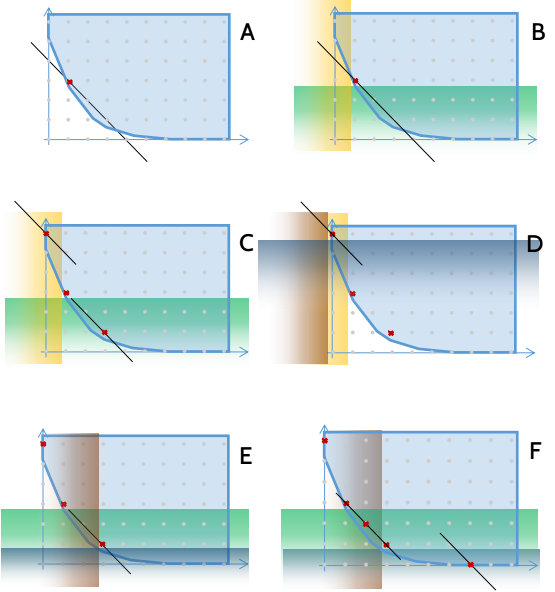
\includegraphics[scale=1]{example.png}
	\end{figure}
	\medskip
	
	\noindent \framebox[\textwidth]{\parbox{0.95\textwidth}{
			\par
			\centerline{\bf Frontier Partitioner Algorithm}
			\par
			\smallskip   		
			\begin{description}
				\smallskip
				\item{\bf Initialization} $k = 0$, ${\cal P}_0 = {\cal P}$, ${\cal D}= {\cal P}_0 $, ${\cal Y} = \emptyset$.
				\item{\bf  While} ${\cal D} \neq \emptyset$
				\smallskip
				\begin{description}
					\item{\bf Take} $\hat{{\cal P}} \in \cal D$, called $\hat{\X}$ its feasible set.
					\item{\bf Solve} $s(\hat{{\cal P}})$.
					\item{\bf If} $s(\hat{{\cal P}})$ is not feasible, then ${\cal D}\smallsetminus \left\{\hat{\cal P}\right\}$ .
					\item{\bf Else} 
					\begin{description}
						 \item{\bf Take} one of its solutions $\hat{x} \in \arg \ds s(\hat{{\cal P}})  $ and call $\hat{f} = f(\hat{x})$.
					\item{\bf Add Cuts} \begin{description}
						\item{\bf For} $h = 1,2$
						\begin{description}
						\item $\X_{k+h} = \X_{k} \cap \left\{x \in \setZn :f_h( x) \le \hat{f}_h -\epsilon_h  \right\}$
						\item ${\cal P}_{k+h} =  \ds \min_{x \in \hat{\X}_{k +h}} f(x) $
						\end{description}
						\item{\bf End For}
						\item $k \rightarrow k+2$
					\end{description}
					\item ${\cal Y} \cup \left\{\hat{f}\right\}$
					\item ${\cal D} \smallsetminus \left\{\hat{\cal P}\right\}$
					\end{description}
				\end{description}
				\item{\bf End While}
				\item\textbf{Return}  $\cal Y$
			\end{description}
		}} 
		\medskip
		
		The main algorithm will work in a setting of global optimality of the Pareto front, since the basic technique used to perform those points always return a Pareto point.
		
		So if we suppose Convex Problems we will have no local Pareto points, then globally our idea is applicable.
		
		The basic problem is
		$$
		\left\{
		\begin{array}{rl}
		\min & f(x) \\
		s.t.& x \in \X
		\end{array}
		\right.
		$$
		
		The difficulty here is to determine the value of the $\epsilon_h$ values. The hard problem of find such a value can be rewritten as
		$$
		\left\{
		\begin{array}{rl}
		\max & f(\hat{x})-f(x) \\
		s.t.& f_h(x) < f_h(\hat{x})\\
		& x \in \X
		\end{array}
		\right.
		$$
		
		Where $f(x): \setZn \rightarrow \setR^m$ is a multidimensional convex function and $\X \subseteq \setZn$ is a convex set.
		
		We do not need to discuss that this problem is NP-Hard, and its relaxation have not a solution. 
		This lead to the definition of properties  the problem has to verify to guarantee the exactness of FPA.
		
		In the following we shows the fundamental properties fo $\epsilon_h$.
		\begin{definition}[Valid value]\label{prop:gammah}
			$\epsilon_h $ is said to be \textbf{valid} if
			$\epsilon_h \in \left(0, \gamma_h \right]$ where $\gamma_h \in \setR : | f_h(x) - f_h(y) | \ge \gamma_h > 0, \ \ \forall \ x,y \in \X : f_h(x) \neq f_h(y) $
		\end{definition}
		
			In some special cases we can easily verify the previous property.
				
			
						
		
	
		\begin{proposition}\label{prop:suffcond}
			If the objective function is such that $ f_h(x):\setZn \rightarrow \setZ$ then $\epsilon_h = 1$ is valid.
			
			\red{ If given a set ${\cal F} \subseteq \setZn$ we have $ f_h({\cal F}) \subseteq \setZ$ then we can use $\epsilon_h = 1$. migliore formulazione}
		\end{proposition}
		\begin{proof}
			Since $f(\X) = \setZ$ then $ | f_h(x) - f_h(y) | \ge 1, \ \ \forall \ x,y \in \X : f_h(x) \neq f_h(y) $ and we can apply proposition \ref{prop:gammah}.
		\end{proof}

		Given a  quadratic function $f_h(x) = x^\intercal Q x + d^\intercal x $, if $Q\succcurlyeq 0 $, $Q \in {\setZ}^{n\times n}$ and $d \in \setZ$ then proposition \ref{prop:suffcond} is verified.
		
	    \begin{proposition}
	    	Given a  quadratic function $f_h(x) = x^\intercal Q x + d^\intercal x $, if $Q\succcurlyeq 0 $, $Q \in \mathbb{ Q}^{n\times n}$ and $d \in \mathbb{Q}$ then $\ds \exists n \in \setN : \epsilon_h = \frac{1}{n}$ is valid.
	    \end{proposition}
	    \begin{proof}
	    	Since $Q \in \mathbb{ Q}^{n\times n}$ and $d \in \mathbb{Q}$ then $ \ds \exists n \in \setN : nQ \in {\setZ}^{n\times n}$ and $nd \in \setZ$. 
	    	
	    	Consider now the function $g_h(x) = x^\intercal nQ x + nd^\intercal x = n f_h(x)$, it verifies proposition \ref{prop:suffcond} and then we can write
	    	$$
	    	\begin{array}{c}
	    	 | g_h(x) - g_h(y) | \ge 1, \ \ \forall \ x,y \in \X : g_h(x) \neq g_h(y) \\
	    	 \Updownarrow
	    	 \\
	    	  | f_h(x) - f_h(y) | \ge \frac{1}{n}, \ \ \forall \ x,y \in \X : f_h(x) \neq f_h(y) 
	    	\end{array}
	    	$$
	    \end{proof}
	    
	    We can make the same considerations considering linear functions, which are special cases with ${\cal Q} : q_{i j} = 0$.
	    
	    
	    
	    \begin{definition}[Limited Frontier]
	    	A problem $\cal P$ is said to have a limited Pareto frontier if the Pareto frontier  is a limited set.
	    \end{definition}
	    
	    
	    We want to remark the following property: Given $a,$ $b,$ $c \in \setR$, if $ a \le b \le c$ then $|b| \le \max\left\{|a|,|c| \right\}$.\footnote{ In fact, if  $b \ge 0$ then $c \ge b \ge 0$ $\Rightarrow$ $|c| \ge |b|$.
	    	
	    	If  $b \le 0$ then $a \le b \le 0$ $\Rightarrow$ $-a \ge -b \ge 0$ $\Rightarrow$ $|a| \ge |b|$.}
	    \begin{proposition}[Sufficient condition of Limited Pareto Frontier]
	    	The Pareto Frontier is limited if  $\omega^h \in \setR^m$, for $h = 1,2$.
	    	
	    	Where $\omega^h = f(\hat{x}^h)$ and
	    	$ \hat{x}^h \in \ds \arg\min_{x \in \X} f_h(x)$.
	    \end{proposition}
	    Before proving this proposition observe that by this definition $ \omega^h_h = z_h^I$, said the ideal value for the $h$-function.
	    \begin{proof}
	    	We call $\cal S$ the set of Pareto points in the space of the objective functions. Knowing the definition of $\omega^h$ we have that for a given point $s \in \cal S$ the following holds
	    	$$s_h \ge \omega_h^h,\  \ h = 1,2$$
	    	On the other hand, since $s$ is a point of the Pareto frontier, then its other component must be at least better than the other one of the $\omega$-points, in formulas
	    	$$s_k \le w_k^h, \ \ h = 1,2,\ k=1,2,\ k\neq h$$
	    	Then we obtain 
	    	$$ \begin{array}{cl}
	    	w_h^h \le s_h \le w^k_h,&\ \ h = 1,2,\ k=1,2,\ k\neq h \\
	    	\Downarrow \\
	    	|s_h| \le \ds\max\left\{|w_h^h|, |w_h^k|\right\} = val_h,& \ \  h = 1,2,\ k=1,2,\ k\neq h\\
	    	\Downarrow \\
	    	|s_h|^2 \le val_h^2,& \ \  h = 1,2,\ k=1,2,\ k\neq h\\
	    	\Downarrow \\
	    	||s||_2 = \ds\sqrt{\sum_h{|s_h|^2}} \le \sqrt{\sum_h{val_h^2}} = val  
	    	\end{array}$$
	    	Thus $\cal S$ is a limited set.
	    \end{proof}
	    \medskip
	    
	    In the following we show that the limitedness of the Pareto Frontier under certain hypothesis implies its finiteness.
	    
	    \begin{proposition}[Sufficient condition for the finiteness of the Pareto Frontier]
	    	If the Pareto frontier is limited, the feasible set $\X$ is a subset of $\setZn$, the objective functions are continuous \red{sempre definite} over $\setRn$  and a valid value $\epsilon_h$ (see definition \ref{prop:gammah}) exists for each objective function, then the Pareto Frontier is finite.
	    \end{proposition} 
	    \begin{proof}
	    	Call $\cal S$ the Pareto Frontier.
	    	
	    	Since the frontier is limited we have $\ds \exists\ M>0, M \in \setR \ : \ ||f(x)||_2 < M, \ \forall f(x) \in \cal S$.
	    	
	    	Since the objectives are continuous over $\setRn$, we can define the following quantities 
	    	$$
	    	\begin{array}{l}
	    	  M_h = \ds \max \left\{ f_h(x) \ :\  ||f(x)||_2 \le M, \ x \in \setRn \right\} < \infty\\
	    	  m_h = \ds \min \left\{ f_h(x) \ :\  ||f(x)||_2 \le M, \ x \in \setRn \right\} > -\infty
	    	\end{array}
	    	$$
	    	
	      Call $\epsilon = \ds \min_{h=1,\dots,m}\left\{ \epsilon_h\right\}	$ with the property 
	      $$ ||p_1 - p_2||_2 \ge \epsilon$$
	      
	      
	      Then each objective $f_h(x)$ can at most assume $\ds \frac{|M_h - m_h|}{\epsilon}$ values. So the maximum number of possible points in the frontier is given by $\ds \frac{1}{\epsilon^m} \prod_{h=1}^m  |M_h - m_h| < \infty$.
	    \end{proof}
	    
	    \begin{proposition}[Sufficient condition for the finiteness of the Pareto Frontier]
	    	If the feasible set $\X$ is finite, then the Pareto Frontier is finite.
	    \end{proposition}
	    \begin{proof}
	    	If $\zeta = \left\lvert \X \right\rvert < \infty$ then $\left\lvert E \right\rvert \le \zeta < \infty$, so the Pareto Frontier has no more points  than $\zeta$.
	    \end{proof}
	    \medskip
	    
	    
	    The fundamental result of FPA is it is possible to prove that in the end all the Pareto frontier will be analyzed without overlapping between subproblems.
	    
	    \begin{theorem}
	    	Given a valid value for $\epsilon_1$ and $\epsilon_2$ and a finite frontier then the 
	    	FPA returns all the Pareto points.
	    \end{theorem}
	    \begin{pf}
	    	Suppose now that $\X^k$ is such that $\hat{x}_k \in arg s_k\left( f(x) \right)$ is a point of the Pareto front. 
	    	
	    	The new problems $k+1$ and $k+2$ are
	    	$$\X^{k+1} = \left\{ x \in \X^k \ : \ f_1(x) \le f_1(\hat{x}_k) - \epsilon_1  \right\}
	    	$$
	    	$$\X^{k+2} = \left\{ x \in \X^k \ : \ f_2(x) \le f_2(\hat{x}_k) - \epsilon_2  \right\}
	    	$$
	    	
	    	We have 
	    	 $$\X^{k+1} \cap \X^{k+2} = \left\{ x \in \X^k \ : \ f_k(x) \le f_k(\hat{x}_k) - \epsilon_k,\ k=1,2 \right\}  \ =\ \emptyset  
	    	$$
	    	In fact if $\ds \exists \ \tilde{x} \in \X^{k+1} \cap \X^{k+2} \ \Rightarrow\ \tilde{x} \preceq \hat{x}_k$ and definitely this implies $\hat{x}_k$ is not part of the Pareto front, on opposite to our assumption about $ arg s_k\left( f(x) \right)$.
	    	
	    	Let now define the set of all points dominated by $\hat{x}_k$
	    	$$\tilde{\X}^{k}= \left\{ x \in \X^k \ : \ f_k(x) \ge f_k(\hat{x}_k) ,\ k=1,2 \right\}  \ =\ \emptyset  
	    	$$
	    	
	    	Its easy to see the family $\tilde{\X}^k,\ \X^{k+1},\ \X^{k+2}$ is a partition\footnote{Given a set ${\cal A}\subseteq \setRn$ a family ${\cal B}_1,\ {\cal B}_1,\dots,\ {\cal B}_q $ is a partition if 
	    		$$
	    		\begin{array}{l}
	    		{\cal B}_i\subseteq {\cal A}, \ i = 1, \dots, q
	    		\\{\cal B}_i \cap {\cal B}_j = \emptyset, \ i = 1, \dots, q,\ i = 1, \dots, q,\ i\neq j
	    		\\ \bigcup_{i=1}^q {\cal B}_i = {\cal A}
	    		\end{array}
	    		$$ 
	    		} of $\X^k$.
	    		
	    	For a fixed $i \in \left\{1,2\right\} $ one of the two sentences is true
	    	\begin{enumerate}
	    		\item $\X^{k+i} \ = \ \emptyset$
	    		\item $\hat{x}_{k+i} \in \arg s_{k+i}\left( f(x)\right)$ is on the frontier
	    	\end{enumerate}
	    	
	    	If $\X^{k+i}$ is empty there will be no points and neither anyone on the frontier.
	    	
	    	
	    	\medskip
	    	To prove the second part we
	    	 need to prove that if $\hat{x}_{k+i} \in E_{k+i}$ then $\hat{x}_{k+i} \in E_{k}$.
	    	
	    	Suppose now by contradiction that $\hat{x}_{k+i} \notin E_{k}$, then $\exists \bar{x} \in \X_k$ such that $\bar{x} \preceq \hat{x}_{k+i}$. This implies that
	    	$$\bar{x} \ : \ \left\{\begin{array}{l}
	    	f_{-i}(\bar{x}) \le f_{-i}(\hat{x}_{k+i})\\
	    	f_{i}(\hat{x}) \le f_{i}(\hat{x}_{k+i})
	    	\end{array} \right.
	    	$$ with one of the two inequalities strict.
	    	
	    	
	    	\medskip
	    	 We also know that $\hat{x}_{k+i} \in \X_{k+i}$ so the second inequality becomes $f_{i}(\hat{x}) \le f_{i}(\hat{x}_{k+i}) \le  f_{i}(\hat{x}_{k}) - \epsilon_i$ thus $\bar{x} \in \X_{k+i}$. This is in contradiction with the fact that $\hat{x}_{k+i} \in E_{k+i}$.
	    	 
	    	 
	    		\medskip
	    	So by the end we have $\hat{x}_{k+i} \in E_k$ for all $k$ and $i$.
	    	
	    	
	    	\medskip
	    	By induction we have that if $\hat{x}_{k+i} \in E_k$ then $\hat{x}_{k+i} \in E_{\hat{k}}$, where $\hat{k}$ is the iteration generating $k$-th problem, indeed $\hat{k} \ : \ \exists \ i \in \left\{ 1, 2\right\} : \hat{k}+i = k$.
	    	
	    	
	    	There is only one generator node $E_0 = E$ for all the subproblems so we can conclude that $\hat{x}_{k+i} \in E$.
	    	
	    	
	    	\medskip
	    	Since our hypothesis on the scalarization algorithm used, when $\X^{k+i} \ \neq \ \emptyset$  we have that  $$\hat{x}_{k+i} \in \arg s_{k+i}\left( f(x)\right) \subseteq E_{k+i} \ \Rightarrow \ \hat{x}_{k+i} \in E$$
	    	
	    	
	    	\medskip
	    	We now must show that we will find all the points of the Frontier.
	    	
	    	To continue with the proof let us show some points \red{scritto male}
	    	\begin{enumerate}
	    		\item A composition of partitions is a partition.
	    		
	    		In other words suppose to have a set $A$ and a partition $\left\{B_j\right\}$ with $j = 1, \dots , n$. Suppose now to have for a certain set $B_j$ a partition $\left\{ C_h \right\}$ with $h= 1,\dots,m$. Then it is trivial to show that the family $\left\{B_1, B_2, \dots, B_{j-1}, C_1, \dots, C_m, B_{j+1}, \dots , B_n \right\}$ is a partition of $A$.
	    		
	    		\item Every time in the algorithm we split the $k$-th set, we have shown we create a partition of the set. In formulas  $\left\{   \tilde{\X}^k,\ \X^{k+1},\ \X^{k+2} \right\}$ is a partition of $\X_k$.
	    		
	    		\item At the end of the algorithm we have a family of sets of the form $\left\{\tilde{\X}_k  \right\}$ with $k \in {\cal K} = \left\{ k \in \setN \ : \ \exists \ \hat{x}_{k} \in \arg s_{k} (f(x)) \right\}$. In fact if a set of the form $\X_{k+i}$ is nonempty, then we can find another point $\hat{x}_{k+i}$ and split again nad so the algorithm can continue.
	    		
	    		\item For what we have just shown every time we find a new point it is on the frontier. Since the frontier is finite we cannot find more points than the ones on the frontier. So by the end we have a bound on the cardinality  $\left\lvert\left\{\tilde{\X}_k  \right\}\right\rvert < \infty$.
	    	\end{enumerate} 
	    	
	    	Suppose now that exists a point on the frontier that our algorithm is not able to find. So suppose $\exists \bar{x} \in \X \ : \ \nexists \ k \in {\cal K} \ : \ f(\bar{x}) = s_k (f(\hat{x}_k))$.
	    	
	    	Combining point 1, 2, 3 and 4 we have that  $\left\{\tilde{\X}_k  \right\}$ is a partition of $\X$, implying
	    	
	    	$$\ds \bar{x} \in \X \ \Rightarrow \ \bar{x} \in \ds\bigcup_{k \in \cal K}  \tilde{\X}_k  \ \Rightarrow \ \exists \ k \in {\cal K} \ : \bar{x} \in \tilde{\X}_k  \ \Rightarrow \ \ \exists \ k \in {\cal K} \ :f(\bar{x}) \ge s_k (f(\hat{x}_k))$$
	    	
	    	in contradiction with what just said.
	    \end{pf}
	    
	    Another important result is given by the fact that we already know how many subproblems will be solved during the computation.
	    \begin{theorem}
	    	Suppose to have a Pareto Frontier with exactly $m$ points, then the FPA algorithm will solve exactly $2 m + 1 $ subproblems and $m + 1$ of them have empty feasible set.
	    \end{theorem}
	    \begin{proof}
	    	From the previous theorem we know that the algorithm ends finding all the Pareto frontier and returning the partition $\left\{\tilde{\X}^k  \right\}$ of the feasible set $\X$. A set $\tilde{\X}^k$ is generated with other sets forming a partition of  $\X^k$, the three sets are  $\left\{   \tilde{\X}^k,\ \X^{k+1},\ \X^{k+2} \right\}$. So by the end we have $3m$ sets generated by the algorithm. The algorithm solves integer programs only on sets of the form $ \X^{k+1}$ and $ \X^{k+2}$, so in the end we have exactly $2m$ problems plus the root one. So the total number of problems solved is $2m + 1$.
	    \end{proof}
	    
	    \section{Equivalence}
	    \begin{equation}\label{simple}
	    \left\{
	    \begin{array}{rl}
	    \min & f(x) \\
	    s.t.& x \in \X
	    \end{array}
	    \right.
	    \end{equation}
	    Where $f:\X \rightarrow \setR^m$  and $\X$ are such that our optimization process can always find the global optimum (e.g. Integer Programming and Convex Programming).
	    
	    Now formulate the problem
	     \begin{equation}\label{modified}
	     \left\{
	     \begin{array}{rl}
	     \min & t \\
	     s.t. & t \ge f(x)\\
	     & x \in \X
	     \end{array}
	     \right.
	     \end{equation}
	     Where $f:\X \rightarrow \setR^m$  and $\X$ are the same of \eqref{simple}.
	    
	    
	    \begin{proposition}
	    	$\hat{x} \in { E}_{\ref{simple}} \ \Rightarrow \ \exists\  \hat{t} \in \setR^m : (\hat{t}, \hat{x}) \in { E}_{\ref{modified}}$
	    	and vice versa
	    	$\ (\hat{t}, \hat{x}) \in { E}_{\ref{modified}} \ \Rightarrow\ \hat{x} \in { E}_{\ref{simple}}$
	    \end{proposition}
	    \begin{proof} We split the proposition into two parts.
	    \medskip
	    
	    	\textit{Part I}. 	$\hat{x} \in { E}_{\ref{simple}} \ \Rightarrow \ \exists\  \hat{t} \in \setR^m : (\hat{t}, \hat{x}) \in { E}_{\ref{modified}}$.
	    	
	    	Call $\hat{t} = f(\hat{x})$. Chosen $\hat{x} \in \X$, since $t \ge f(\hat{x}) = \hat{t}$ then $\nexists \ t \in \setR^m : t \neq \hat{t}, \ t \preccurlyeq \hat{t}$. \footnote{$\nexists \ t \in \setR^m : t \le \hat{t},\ t \neq \hat{t}$.}
	    	
	    	Since $\hat{x} \in E_{\ref{simple}}$ then $\nexists\ x \in \X : f(x) \preccurlyeq f(\hat{x})$ thus $\nexists\ x \in \X,\  t \in \setR^m : t \neq \hat{t},\ \hat{t} = f(\hat{x}) \ge t \ge f(x), \ f(x) \neq f(\hat{x}) \ \Rightarrow (\hat{t}, \hat{x}) \in E_{\ref{modified}}$.
	    	\medskip
	    	
	    	 \textit{Part II}. $(\hat{t}, \hat{x}) \in { E}_{\ref{modified}} \ \Rightarrow\ \hat{x} \in { E}_{\ref{simple}}$.
	    	 
	    	 We start proving 
	    	 \begin{equation}\label{teq}
	    	 (\hat{t},\hat{x}) \in E_{\ref{modified}} \ \Rightarrow\ \hat{t} = f(\hat{x})
	    	 \end{equation}
	    	 
	    	  In fact by contradiction suppose  $(\hat{t},\hat{x}) \in E_{\ref{modified}}$ and $\hat{t} \neq f(\hat{x})$, implying $\hat{t} > f(\hat{x})$. We can build the feasible point $\tilde{t} = f(\hat{x})$, obtaining $f(\hat{x}) = \tilde{t} < \hat{t} \ \Rightarrow\  \tilde{t} \preccurlyeq \hat{t}$ denying  the fact that $(\hat{t},\hat{x}) \in E_{\ref{modified}}$.
	    	 \medskip 
	    	 
	    	 Now since we know that $\ (\hat{t}, \hat{x}) \in { E}_{\ref{modified}} $ we have that $\nexists\ (t,x) \in {\cal G}(x)\times \X : t \preccurlyeq \hat{t}$, where ${\cal G}(x) = \left\{t \in \setR^m : t \ge f(x)  \right\}$.
	    	 Taking into account \eqref{teq} we have that
	    	 $\nexists\ (t,x) \in {\cal G}(x)\times \X : f(x) \le t \preccurlyeq \hat{t} = f(\hat{x})$.
	    	 
	    	 We want to show that 
	    	 $$
	    	 \begin{array}{c}
	    	 \nexists\ (t,x) \in {\cal G}(x)\times \X : f(x) \preccurlyeq  f(\hat{x})\\
	    	 \Downarrow\\
	    	 \nexists\ x \in \X : f(x) \preccurlyeq  f(\hat{x})
	    	 \end{array}
	    	 $$
	    	 By contradiction suppose that $\exists\ x \in \X : f(x) \preccurlyeq  f(\hat{x})$ but then there is a point $(t=f(x), x) \in {\cal G}(x) \times \X : f(x) \preccurlyeq f(\hat{x})$, and this is not possible.
	    \end{proof}
	    
	    
	    \section{Heuristic for Convex Problems}
	    Even in the quadratic case once we have determined the constraint to add to the formulation, then the resulting problem is Quadratic Objective Quadratically Constrained Integer program.
	    
	    In general could be useful to use an heuristic which does not increment the difficulty of the feasible set.
	    
	    Since we are supposing Convex objectives, once we know a value for $\epsilon_h$ (or an estimation) and comparison point $\hat{x}$, we can write
	    $$
	    \begin{array}{c}
	    f_h(x) \le f_h(\hat{x}) - \epsilon_h\\\Downarrow\\
	    \nabla f_h(\hat{x})^\intercal \left(\hat{x} - y \right) \ge f_h(\hat{x}) - f_h(x)\ge \epsilon_h
	    \end{array}
	    $$
	    
	    We use this linearized constraints to reduce the hardness of the formulation.
	    
	    \section{Computational Experience}
	    
	    The focus of this section is on linear problems since we can mae a comparison between different methods. In particular we will provide results for FPA algorithm and the one proposed by Mavrotas in \cite{calippo}. There is no 
	    
	    \begin{table}[]
	    	\footnotesize
	    	\centering
	    	\caption{My caption}
	    	\label{table1}
	    	\begin{tabular}{ccccccccccccc}
	    		\multicolumn{1}{l}{}            & \multicolumn{4}{|c|}{Frontier Partitioner Algorithm Time (ms)}                                                          & \multicolumn{4}{c|}{Mavrotas Algorithm Time (ms) }                                                                      \\ \hline
	    		\multicolumn{1}{c|}{Experiment} & \multicolumn{1}{c|}{Average} & \multicolumn{1}{c|}{Std Dev} & \multicolumn{1}{c|}{Max} & \multicolumn{1}{c|}{Min} & \multicolumn{1}{c|}{Average} & \multicolumn{1}{c|}{Std Dev} & \multicolumn{1}{c|}{Max} & \multicolumn{1}{c|}{Min} \\ \hline
	    		10     x 10   x 0   & 166.5                        & 307.88            & 1038.0                   & 25.0                     & 219.2                        & 66.35           & 339.0                    & 138.0                    \\
	    		10     x 10   x 1   & 117.9                        & 39.83           & 188.0                    & 68.0                     & 181.2                        & 23.69           & 230.0                    & 148.0                    \\
	    		10     x 10   x 2   & 148.3                        & 212.27           & 668.0                    & 35.0                     & 187.2                        & 44.97            & 280.0                    & 131.0                    \\
	    		10     x 10   x 3   & 104.1                        & 65.62            & 228.0                    & 24.0                     & 161.9                        & 34.74           & 214.0                    & 103.0                    \\
	    		10     x 10   x 4   & 82.6                         & 50.84            & 186.0                    & 16.0                     & 183.1                        & 47.64           & 284.0                    & 114.0                    \\
	    		10     x 10   x 5   & 108.1                        & 88.82          & 321.0                    & 50.0                     & 177.3                        & 37.81            & 239.0                    & 119.0                    \\
	    		10     x 10   x 6   & 124.3                        & 117.78           & 360.0                    & 24.0                     & 202.8                        & 51.14            & 314.0                    & 122.0                    \\
	    		10     x 10   x 7   & 96.9                         & 75.49            & 271.0                    & 30.0                     & 162.4                        & 27.45           & 203.0                    & 125.0                    \\
	    		10     x 10   x 8   & 90.6                         & 53.35          & 170.0                    & 28.0                     & 163.4                        & 42.34            & 222.0                    & 92.0                     \\
	    		10     x 10   x 9   & 94.7                         & 65.33            & 230.0                    & 31.0                     & 174.3                        & 48.60           & 257.0                    & 90.0                     \\
	    		20     x 10   x 0   & 250.7                        & 186.44           & 577.0                    & 44.0                     & 2590.4                       & 624.74            & 3618.0                   & 1729.0                   \\
	    		20     x 10   x 1   & 627.6                        & 694.11            & 2476.0                   & 117.0                    & 3124.9                       & 888.01            & 4427.0                   & 1489.0                   \\
	    		20     x 10   x 2   & 437.9                        & 189.45           & 712.0                    & 157.0                    & 3028.2                       & 644.90            & 4165.0                   & 2184.0                   \\
	    		20     x 10   x 3   & 419.2                        & 673.93             & 2304.0                   & 65.0                     & 2731.8                       & 624.99            & 3528.0                   & 1939.0                   \\
	    		20     x 10   x 4   & 896.3                        & 830.70         & 2588.0                   & 45.0                     & 3082.4                       & 790.46            & 4255.0                   & 1749.0                   \\
	    		20     x 10   x 5   & 665.4                        & 641.08             & 1949.0                   & 29.0                     & 4614.4                       & 1713.32          & 7589.0                   & 2472.0                   \\
	    		20     x 10   x 6   & 606.5                        & 384.94           & 1170.0                   & 27.0                     & 3109.8                       & 841.21            & 4344.0                   & 1947.0                   \\
	    		20     x 10   x 7   & 857.3                        & 828.58            & 2932.0                   & 119.0                    & 3350.1                       & 1151.39         & 5542.0                   & 1533.0                   \\
	    		20     x 10   x 8   & 394.6                        & 321.91           & 1168.0                   & 107.0                    & 2988.5                       & 645.95            & 4186.0                   & 1940.0                   \\
	    		20     x 10   x 9   & 496.7                        & 390.92           & 1323.0                   & 91.0                     & 3227.5                       & 867.74           & 4936.0                   & 1776.0                   \\
	    		30     x 10   x 0   & 1665.2                       & 1474.33            & 4313.0                   & 226.0                    & 18946.5                      & 3936.56          & 24517.0                  & 13080.0                  \\
	    		30     x 10   x 1   & 1646.1                       & 1435.61           & 4366.0                   & 166.0                    & 18728.1                      & 5238.12            & 30539.0                  & 9928.0                   \\
	    		30     x 10   x 2   & 1623.9                       & 1304.13           & 3853.0                   & 477.0                    & 19658.1                      & 5548.89            & 25602.0                  & 10230.0                  \\
	    		30     x 10   x 3   & 3051.2                       & 2162.46          & 6631.0                   & 38.0                     & 20013.9                      & 3703.17          & 25259.0                  & 14154.0                  \\
	    		30     x 10   x 4   & 1865.5                       & 1433.32          & 4004.0                   & 307.0                    & 18737.6                      & 3993.58           & 25010.0                  & 13423.0                  \\
	    		30     x 10   x 5   & 1791.0                       & 1394.81           & 4693.0                   & 386.0                    & 17647.8                      & 4006.52            & 23196.0                  & 12072.0                  \\
	    		30     x 10   x 6   & 885.7                        & 605.58            & 2046.0                   & 181.0                    & 21776.9                      & 8875.90            & 37929.0                  & 11805.0                  \\
	    		30     x 10   x 7   & 1686.1                       & 1472.15         & 5016.0                   & 105.0                    & 19972.9                      & 4039.23            & 27119.0                  & 14916.0                  \\
	    		30     x 10   x 8   & 1858.1                       & 1251.97           & 3545.0                   & 200.0                    & 18225.1                      & 5623.28            & 25606.0                  & 11001.0                  \\
	    		30     x 10   x 9   & 2304.7                       & 2038.46           & 6645.0                   & 149.0                    & 21160.8                      & 6340.89            & 31024.0                  & 13923.0                 
	    	\end{tabular}
	    \end{table}
	    
	    \begin{figure}
	    	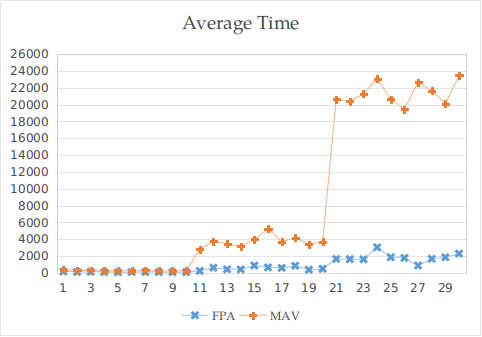
\includegraphics[height=5cm]{reslin.png}
	     	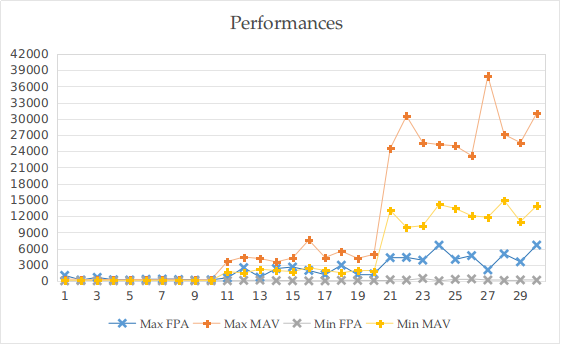
\includegraphics[height=5cm]{reslinminmax.png}
	     \end{figure}
	     
	     \begin{table}[]
	     	\footnotesize
	     	\centering
	     	\caption{My caption}
	     	\label{table2}
	     	\begin{tabular}{cccccccccccc}
	     		\multicolumn{4}{|c|}{Pareto Points}                                                                             & \multicolumn{4}{c|}{FPA Number of nodes}                                                                       & \multicolumn{4}{c|}{MAV Number of nodes}                                                                       \\ \hline
	     		\multicolumn{1}{|c|}{Average} & \multicolumn{1}{c|}{Std Dev} & \multicolumn{1}{c|}{Max} & \multicolumn{1}{c|}{Min} & \multicolumn{1}{c|}{Average} & \multicolumn{1}{c|}{Std Dev} & \multicolumn{1}{c|}{Max} & \multicolumn{1}{c|}{Min} & \multicolumn{1}{c|}{Average} & \multicolumn{1}{c|}{Std Dev} & \multicolumn{1}{c|}{Max} & \multicolumn{1}{c|}{Min} \\ \hline
	     		4.1                        & 1.85                         & 7.0                      & 1.0                      & 8.2                       & 3.71                         & 14.0                     & 2.0                      & 422.4                     & 101.20                       & 668.0                    & 314.0                    \\
	     		4.9                        & 1.10                         & 7.0                      & 3.0                      & 9.8                       & 2.20                         & 14.0                     & 6.0                      & 406.8                     & 56.25                        & 518.0                    & 316.0                    \\
	     		4.4                        & 1.58                         & 7.0                      & 2.0                      & 8.8                       & 3.16                         & 14.0                     & 4.0                      & 425.6                     & 108.77                       & 672.0                    & 300.0                    \\
	     		4.3                        & 1.89                         & 7.0                      & 2.0                      & 8.6                       & 3.78                         & 14.0                     & 4.0                      & 365.4                     & 78.93                        & 486.0                    & 230.0                    \\
	     		4.3                        & 1.64                         & 7.0                      & 2.0                      & 8.6                       & 3.27                         & 14.0                     & 4.0                      & 417.0                     & 114.29                       & 662.0                    & 252.0                    \\
	     		4.2                        & 1.48                         & 7.0                      & 2.0                      & 8.4                       & 2.95                         & 14.0                     & 4.0                      & 391.6                     & 86.18                        & 540.0                    & 256.0                    \\
	     		5.4                        & 2.07                         & 9.0                      & 3.0                      & 10.8                      & 4.13                         & 18.0                     & 6.0                      & 455.2                     & 124.29                       & 750.0                    & 276.0                    \\
	     		4.9                        & 2.33                         & 10.0                     & 2.0                      & 9.8                       & 4.66                         & 20.0                     & 4.0                      & 367.2                     & 68.11                        & 472.0                    & 280.0                    \\
	     		5.1                        & 2.73                         & 12.0                     & 2.0                      & 10.2                      & 5.45                         & 24.0                     & 4.0                      & 370.2                     & 96.98                        & 508.0                    & 210.0                    \\
	     		3.6                        & 1.78                         & 6.0                      & 1.0                      & 7.2                       & 3.55                         & 12.0                     & 2.0                      & 395.6                     & 116.09                       & 594.0                    & 206.0                    \\
	     		5.1                        & 1.97                         & 7.0                      & 2.0                      & 10.2                      & 3.94                         & 14.0                     & 4.0                      & 3496.0                    & 867.18                       & 4952.0                   & 2368.0                   \\
	     		6.7                        & 2.36                         & 11.0                     & 3.0                      & 13.4                      & 4.72                         & 22.0                     & 6.0                      & 4274.8                    & 1248.80                      & 6186.0                   & 2022.0                   \\
	     		7.2                        & 2.10                         & 10.0                     & 3.0                      & 14.4                      & 4.20                         & 20.0                     & 6.0                      & 4170.8                    & 872.65                       & 5808.0                   & 2924.0                   \\
	     		6.7                        & 2.16                         & 10.0                     & 3.0                      & 13.4                      & 4.33                         & 20.0                     & 6.0                      & 3741.8                    & 823.48                       & 4882.0                   & 2620.0                   \\
	     		7.1                        & 2.08                         & 10.0                     & 4.0                      & 14.2                      & 4.16                         & 20.0                     & 8.0                      & 4232.8                    & 1100.08                      & 5916.0                   & 2428.0                   \\
	     		6.6                        & 2.95                         & 13.0                     & 2.0                      & 13.2                      & 5.90                         & 26.0                     & 4.0                      & 5282.0                    & 1937.97                      & 8896.0                   & 2998.0                   \\
	     		6.7                        & 2.31                         & 10.0                     & 2.0                      & 13.4                      & 4.62                         & 20.0                     & 4.0                      & 4037.8                    & 985.95                       & 5282.0                   & 2528.0                   \\
	     		6.9                        & 2.96                         & 13.0                     & 4.0                      & 13.8                      & 5.92                         & 26.0                     & 8.0                      & 4470.0                    & 1516.27                      & 7304.0                   & 1998.0                   \\
	     		6.9                        & 2.33                         & 12.0                     & 4.0                      & 13.8                      & 4.66                         & 24.0                     & 8.0                      & 4122.6                    & 930.55                       & 5852.0                   & 2620.0                   \\
	     		6.8                        & 2.49                         & 10.0                     & 4.0                      & 13.6                      & 4.97                         & 20.0                     & 8.0                      & 4407.6                    & 1178.10                      & 6734.0                   & 2512.0                   \\
	     		9.2                        & 3.61                         & 15.0                     & 4.0                      & 18.4                      & 7.23                         & 30.0                     & 8.0                      & 15035.0                   & 3289.55                      & 20074.0                  & 10738.0                  \\
	     		8.7                        & 3.13                         & 15.0                     & 5.0                      & 17.4                      & 6.26                         & 30.0                     & 10.0                     & 14869.4                   & 4249.19                      & 24760.0                  & 8108.0                   \\
	     		8.2                        & 3.55                         & 14.0                     & 4.0                      & 16.4                      & 7.11                         & 28.0                     & 8.0                      & 15317.2                   & 4120.41                      & 20376.0                  & 8062.0                   \\
	     		12.0                       & 5.50                         & 19.0                     & 1.0                      & 24.0                      & 10.99                        & 38.0                     & 2.0                      & 16277.4                   & 2943.17                      & 20772.0                  & 11732.0                  \\
	     		10.4                       & 2.50                         & 14.0                     & 7.0                      & 20.8                      & 5.01                         & 28.0                     & 14.0                     & 15174.0                   & 3363.16                      & 20428.0                  & 10804.0                  \\
	     		7.6                        & 2.41                         & 11.0                     & 4.0                      & 15.2                      & 4.83                         & 22.0                     & 8.0                      & 14350.4                   & 3133.44                      & 18680.0                  & 9984.0                   \\
	     		9.2                        & 3.12                         & 14.0                     & 5.0                      & 18.4                      & 6.24                         & 28.0                     & 10.0                     & 17732.2                   & 7198.87                      & 30698.0                  & 9610.0                   \\
	     		8.7                        & 3.83                         & 14.0                     & 2.0                      & 17.4                      & 7.66                         & 28.0                     & 4.0                      & 16305.6                   & 3308.71                      & 22354.0                  & 12208.0                  \\
	     		9.5                        & 2.95                         & 13.0                     & 5.0                      & 19.0                      & 5.91                         & 26.0                     & 10.0                     & 14874.0                   & 4570.54                      & 20740.0                  & 9142.0                   \\
	     		11.2                       & 4.47                         & 19.0                     & 5.0                      & 22.4                      & 8.93                         & 38.0                     & 10.0                     & 17367.8                   & 5290.21                      & 25890.0                  & 11486.0                 
	     	\end{tabular}
	     \end{table}
	     
	     \begin{table}[]
	     	\footnotesize
	     	\centering
	     	\caption{My caption}
	     	\label{table3}
	     	\begin{tabular}{lcccccccc}
	     		\multicolumn{1}{l|}{}           & \multicolumn{4}{c|}{Time (ms)}                                                                                         & \multicolumn{4}{c|}{Number of Pareto points}                                                                      \\ \hline
	     		\multicolumn{1}{l|}{Experiment} & \multicolumn{1}{c|}{Average} & \multicolumn{1}{c|}{Std Dev} & \multicolumn{1}{c|}{Max} & \multicolumn{1}{c|}{Min} & \multicolumn{1}{c|}{Average} & \multicolumn{1}{c|}{Std Dev} & \multicolumn{1}{c|}{Max} & \multicolumn{1}{c|}{Min} \\ \hline
	     		10 x 10 x 0                     & 343.2                        & 271.58                       & 970                      & 74                       & 3.8                          & 1.55                         & 6                        & 2                        \\
	     		10 x 10 x 1                     & 226.3                        & 120.28                       & 439                      & 60                       & 3.8                          & 1.55                         & 7                        & 2                        \\
	     		10 x 10 x 2                     & 171.3                        & 89.79                        & 344                      & 47                       & 3.2                          & 1.32                         & 5                        & 2                        \\
	     		10 x 10 x 3                     & 486.8                        & 207.89                       & 985                      & 226                      & 5.9                          & 1.6                          & 9                        & 3                        \\
	     		10 x 10 x 4                     & 355.2                        & 260.12                       & 971                      & 83                       & 5.3                          & 2.06                         & 9                        & 3                        \\
	     		10 x 10 x 5                     & 327.9                        & 266.41                       & 845                      & 48                       & 4.5                          & 2.07                         & 8                        & 2                        \\
	     		10 x 10 x 6                     & 529                          & 283.26                       & 1209                     & 292                      & 6                            & 2.31                         & 12                       & 4                        \\
	     		10 x 10 x 7                     & 144                          & 98.9                         & 376                      & 51                       & 3.4                          & 1.17                         & 5                        & 2                        \\
	     		10 x 10 x 8                     & 464.2                        & 259.54                       & 875                      & 170                      & 4.6                          & 1.9                          & 7                        & 2                        \\
	     		10 x 10 x 9                     & 272.1                        & 233.35                       & 723                      & 24                       & 4.3                          & 1.89                         & 8                        & 1                        \\
	     		20 x 10 x 0                     & 1373.7                       & 1013.7                       & 3419                     & 287                      & 6.4                          & 3.17                         & 13                       & 3                        \\
	     		20 x 10 x 1                     & 1391.7                       & 616                          & 2892                     & 774                      & 6.4                          & 1.84                         & 11                       & 4                        \\
	     		20 x 10 x 2                     & 1564.9                       & 1137.5                       & 4212                     & 329                      & 6.6                          & 3.1                          & 12                       & 3                        \\
	     		20 x 10 x 3                     & 1467.5                       & 806.11                       & 2632                     & 313                      & 6.5                          & 2.64                         & 10                       & 3                        \\
	     		20 x 10 x 4                     & 1452                         & 791.69                       & 2827                     & 385                      & 6.1                          & 2.13                         & 10                       & 4                        \\
	     		20 x 10 x 5                     & 1800.3                       & 963.91                       & 4084                     & 666                      & 7.7                          & 2.71                         & 13                       & 4                        \\
	     		20 x 10 x 6                     & 1225.9                       & 472.69                       & 2192                     & 552                      & 5.9                          & 1.73                         & 10                       & 4                        \\
	     		20 x 10 x 7                     & 1316                         & 621.03                       & 2294                     & 333                      & 6.2                          & 1.81                         & 9                        & 4                        \\
	     		20 x 10 x 8                     & 1225.3                       & 513.82                       & 2349                     & 334                      & 5.6                          & 1.35                         & 8                        & 3                        \\
	     		20 x 10 x 9                     & 1532.8                       & 929.24                       & 3406                     & 222                      & 6.6                          & 2.67                         & 10                       & 2                        \\
	     		30 x 10 x 0                     & 3116.6                       & 1414.71                      & 6579                     & 1590                     & 8.8                          & 3.71                         & 18                       & 5                        \\
	     		30 x 10 x 1                     & 3334.3                       & 1713.68                      & 6754                     & 842                      & 9.2                          & 2.82                         & 13                       & 3                        \\
	     		30 x 10 x 2                     & 2753.5                       & 1421.49                      & 6029                     & 1136                     & 7.7                          & 3.23                         & 12                       & 3                        \\
	     		30 x 10 x 3                     & 2572.7                       & 1663.46                      & 6294                     & 557                      & 7.2                          & 3.36                         & 14                       & 2                        \\
	     		30 x 10 x 4                     & 2903.7                       & 2422.01                      & 7911                     & 193                      & 8.4                          & 6.67                         & 22                       & 1                        \\
	     		30 x 10 x 5                     & 3385.4                       & 1734.99                      & 5930                     & 475                      & 8.4                          & 3.92                         & 15                       & 2                        \\
	     		30 x 10 x 6                     & 3248.3                       & 1725.48                      & 6799                     & 458                      & 8.1                          & 3.73                         & 15                       & 1                        \\
	     		30 x 10 x 7                     & 3655.4                       & 3525.51                      & 13027                    & 816                      & 9                            & 5.58                         & 22                       & 3                        \\
	     		30 x 10 x 8                     & 3058.1                       & 881.01                       & 4648                     & 1929                     & 8                            & 1.89                         & 11                       & 5                        \\
	     		30 x 10 x 9                     & 2297.5                       & 966.16                       & 4020                     & 832                      & 6                            & 2.11                         & 10                       & 2                       
	     	\end{tabular}
	     \end{table}
	     
	     \bibliographystyle{apalike}
	     \bibliography{frontierAlg}
	     
\end{document}